% Chapter 2 (from main tex file)
% Research Project
% Author: Javier Reyes

\chapter{Hardware Platform Design}

The workflow for the Zynq-7000 architecture starts with the hardware specification for both PS and
PL technologies. Xilinx provide a complete suite of programs and tools for the entire desing cycle
of the embedded solution, either in a standalone platform or in an embedded OS.

\begin{figure}[htp]
	\centering
	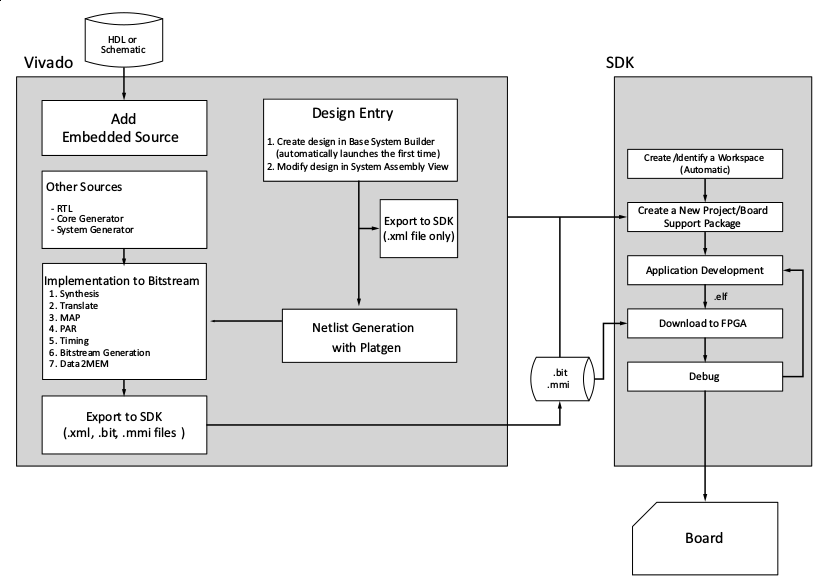
\includegraphics[width=\textwidth]{embedded-flow.png}
	\caption{Embedded Design Process Flow, from \cite{UG1043}.} \label{fig:embedded-flow}
\end{figure}%

The workflow is split into different tools provided by Xilinx. The hardware specific tasks will be
covered in section \ref{hardware-design}. The software component will be covered in chapters
\ref{embedded-linux} and \ref{software-application}.

\section{Hardware Design} \label{hardware-design}

For the definition, configuration and flashing of the FPGA fabric, the Vivado Design Suite includes
the necessary tools. The distribution of tasks and their respective tool scenario is shown in figure
\ref{fig:hardware-tasks-tools}.

\begin{figure}[htp]
	\centering
	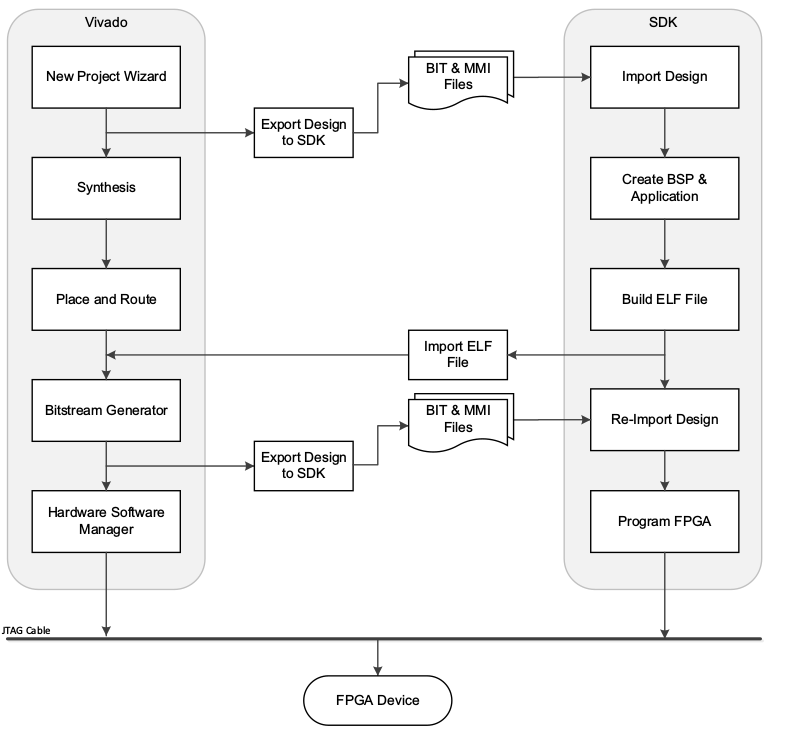
\includegraphics[width=\textwidth]{hardware-tasks-tools.png}
	\caption{Hardware design tasks and tools scenario, from \cite{UG1043}.}
	\label{fig:hardware-tasks-tools}
\end{figure}%

The typical Hardware/Software Co-Design present in the tools allows a continuous verification and
validation of the design. For this project, the process include a third element for building a
custom Linux OS, which will be covered in chapter \ref{embedded-linux}. There are several approaches
to create a hardware definition for the Zynqberry board in the Vivado Desgin Suite, a GUI-based
interaction, or a TCL console.

\subsection{Vivado GUI}

The process for a Zynq-7000 device can be easily done in the Vivado GUI, under Windows or Linux
operative systems. The general procedure can be listed as follows:

\begin{enumerate}
	\item Start the Vivado IDE.
	\item Create New Project.
	\begin{enumerate}
		\item Define Project name and location.
		\item Select RTL project type.
		\item If necessary, add any source files (HDL or constraints).
		\item Select the device as ZYNQ XC7Z010-CLG225-1.
	\end{enumerate}
	\item Create New Block Design.
	\item Add the IP Core for the ZYNQ7 Processing System.
	\item Configure the desired characteristics of the PS and PL.
	\item If necessary, add additional IP Cores, or create own IP Core with HLS (See Appendix
	\ref{appen2}).
	\item Run the Block Automation or Connection Automation if required.
	\item Validate the Block Design.
	\item If necessary, assign the required constraints.
	\item Run the Synthesis, Implementation and Generate Bitstream.
	\item Export the Hardware Platform (including Bitstream).
\end{enumerate}

The general process can contain small variances depending on the specific design. From this point,
the software design can be started, by using the exported hardware definition into the SDK. This
part is expanded in chapter \ref{software-application}.

\subsection{TCL Console}

The entire process made in Vivado GUI can be performed in a TCL console by using text-based scripts.
This makes some environments more adequate for maintainability and expandability, and even
facilitates the use of VCS tools by having the hardware definition described in a text file.

The Vivado core has included a TCL engine, which has been used as an industry standar choice for
scripting and automating software tasks. For a project created using the GUI, actions are displayed
as TCL commands in the TCL console, and the commands are saved in a file \texttt{vivado.jou} and
together with the returned messages in the file \texttt{vivado.log}. A typical project creation
script is shown in snippet \ref{tcl-script}.

\begin{lstlisting}[language=tcl, basicstyle=\scriptsize\ttfamily, tabsize=2,
	commentstyle=\color{darkgray}, keywordstyle=\color{blue}, backgroundcolor=\color{lightgray},
	morekeywords={create_project, add_files, import_files, set_property, update_compile_order,
	launch_runs, wait_on_run, open_run, report_timming_summary, report_power}, breaklines=true,
	numbers=left, float=htb,
	caption={[TCL project creation example]TCL project creation example, from \cite{UG895}},
	label={tcl-script}]
	# Typical usage: vivado -mode tcl -source run_bft_project.tcl
	# Create the project and directory structure
	create_project -force project_bft_batch ./project_bft_batch -part xc7z010-clg225-1
	#
	# Add various sources to the project
	add_files {./Sources/hdl/FifoBuffer.v ./Sources/hdl/async_fifo.v \
	./Sources/hdl/bft.vhdl}
	add_files -fileset sim_1 ./Sources/hdl/bft_tb.v
	add_files ./Sources/hdl/bftLib/
	add_files -fileset constrs_1 ./Sources/bft_full.xdc
	#
	# Now import/copy the files into the project
	import_files -force
	#
	# Set VHDL library property on some files
	set_property library bftLib [get_files {*round_*.vhdl core_transform.vhdl \
	bft_package.vhdl}]
	#
	# Update to set top and file compile order
	update_compile_order -fileset sources_1
	update_compile_order -fileset sim_1
	#
	# Launch Synthesis
	launch_runs synth_1
	wait_on_run synth_1
	open_run synth_1 -name netlist_1
	#
	# Generate a timing and power reports and write to disk
	# Can create custom reports as required
	report_timing_summary -delay_type max -report_unconstrained -check_timing_verbose \
	-max_paths 10 -input_pins -file syn_timing.rpt
	report_power -file syn_power.rpt
	#
	# Launch Implementation
	launch_runs impl_1 -to_step write_bitstream
	wait_on_run impl_1
	#
	# Generate a timing and power reports and write to disk
	# comment out the open_run for batch mode
	open_run impl_1
	report_timing_summary -delay_type min_max -report_unconstrained \
	-check_timing_verbose -max_paths 10 -input_pins -file imp_timing.rpt
	report_power -file imp_power.rpt
	#
	# Can open the graphical environment if visualization desired
	# comment out the for batch mode
	#start_gui
\end{lstlisting}

\section{Block Design}

The design of the hardware portion of the system can be considered in itself a project, and the
complexity of it would make this work out of focus. Therefore, an overview of the tool capabilities
and procedures related is presented.



% TODO: Complete chapter

\subsection{IP Core}

\subsection{High Level Synthesis}
